% Chapter Template

\chapter{Results and Analysis} % Main chapter title

\label{c5} % Change X to a consecutive number; for referencing this chapter elsewhere, use \ref{ChapterX}


%\section{Results and Analysis}

%\subsection{Quantitative Analysis}

\section{Results and Analysis}
The original datasets are used to evaluate four different models on the given performance metrices. ML models like AdaBoost Regressor, CatBoost Regressor, XGBoost Regressor are the models belongs to same class of model with minor differences in approach. ARIMA can also be a time series approach.\cite{pavlyshenko2018using} In our analysis of model for the sales data, it is observed that, multi-view approach can be a good methodology for learning and it outperforms most of the models used comparatively. Apart from proposed framework in this study, It can also be genaralised with other models like, AdaBoost-Multiview, CatBoost-Multiview frameworks and so on. The proposed Mv-XGBr is implemented on the store sales data and produces better results compared to other given base models as in Tables 4, 5, 6 we can see that RMSE for the Mv-XGBr is much effective than those of other models in majority of the cases. The sales data is relatively analysed based on their EDA and the model effectiveness over the data. The used hyperparameters are also mentioned in Table 8. Throughout the study, multi-view learning and its approach remained in the focus. View selection methodology in the form of feature set partitioning studied along with its limitations. Analytically, the comparative representation of proposed framework have been plotted with shown values as empirical data in Tables 4, 5, 6 and 7. The results have been described also in the form of relative percentage changes in the performance. The corresponding percentage changes in RMSE value for proposed and comparative boosting models have been mentioned in Table 9 and 10. The XGBoost model is relatively performing poor but proposed Mv-XGBr method have entirely transformed its result in original dataset X. The minimum RMSE value for XGBoost for original dataset is 48.5781 that belongs to store ID 332. There is a similar kind of outcome can be observed on same data for dataset category $X’$ too. Moreover, the percentage changes even increased to 61.27\% for the same store ID 332  . Comparatively, proposed method performs effectively for atleast one store data relatively with other models. Extra Tree model performs well and is close to the proposed framework predicting capability, on overall data X. Even, it yields better result in two of the store data 357 and  392, but proposed method is able to outperforms it on all others available store data. The relative plotting of the model for the given store data is visualized in Figures 12, 13, 14, 15 and 16. Apart from this, barplot of results for both category of dataset is visualized in Figures 8, 9, 10 and 11. \\
Additionally, in this study, there is a scope of understanding view development and optimization of dataset in both categories. selecting optimal view number for the model is the matter of investigation and analysis. Although the evaluation of views and Mv-XGBr framework has already been described in section 4, but concept of multiview learning cannot be generalised so precisely. It depends upon the individual features of the dataset and its effectiveness.


\begin{table*}[!h]
\centering
\setlength{\tabcolsep}{3pt}
 {\renewcommand{\arraystretch}{1}%
\caption{RMSE of stand alone boosting methods and proposed Mv-XGBr over the multiple stores with original features,(X)}
\label{tab:my-table}
%\resizebox{\textwidth}{!}{%
\begin{tabular}{llllll}
\hline \textbf{Store ID} & \textbf{Extra Tree} & \textbf{AdaBoost} & \textbf{CatBoost} & \textbf{XGBoost} & \textbf{Proposed}    \\ \hline
\textbf{189}   & 46.1702             & 230.5995                      & 131.5315                      & 91.9648                      & \textbf{42.8813}  \\
\textbf{207}   & 109.6315            & 251.2419                      & 223.6635                      & 86.2215                      & \textbf{72.5859}  \\
\textbf{332}   & 28.2175             & 106.1206                      & 76.2900                       & 48.5781                      & \textbf{22.8579}  \\
\textbf{333}   & 57.1537             & 154.8037                      & 133.2245                      & 71.2214                      & \textbf{36.8040}  \\
\textbf{357}   & 36.9128             & 212.1578                      & 104.5226                      & 103.6653                     & 41.0162           \\
\textbf{392}   & 62.4399             & 125.5250                      & 208.9143                      & 103.8443                     & 75.7935           \\
\textbf{405}   & 54.1017             & 94.4884                       & 120.0382                      & 92.4887                      & \textbf{37.1129}  \\
\textbf{489}   & 66.6955             & 282.5370                      & 204.1499                      & 112.6974                     & \textbf{53.6535}  \\
\textbf{492}   & 57.9823             & 179.0433                      & 170.1749                      & 60.1017                      & \textbf{34.6531}  \\
\textbf{504}   & 54.3112             & 103.5482                      & 128.2980                      & 122.7050                     & \textbf{51.5927}  \\ \hline
\end{tabular}%
}
\end{table*}

\begin{table*}[]
\centering
\setlength{\tabcolsep}{3pt}
 {\renewcommand{\arraystretch}{1}%
\caption{RMSE of stand alone boosting methods and proposed Mv-XGBr over the multiple stores with original features,(X')}
\label{tab:my-table}
%\resizebox{\textwidth}{!}{%
\begin{tabular}{llllll}
\hline \textbf{Store ID} & \textbf{Extra Tree} & \textbf{AdaBoost} & \textbf{CatBoost} & \textbf{XGBoost} & \textbf{Proposed}    \\ \hline

\textbf{189}   & 76.4855             & 196.8789                      & 204.2693                      & 113.8798                     & \textbf{56.0571}
           \\
\textbf{207}   & 74.2640             & 220.4196                      & 138.1857                      & 147.9886                     & 79.8944  \\
\textbf{332}   & 25.2038             & 110.2352                      & 65.5687                       & 70.6404                      & 28.3589           \\
\textbf{333}   & 46.2811             & 154.8037                      & 120.0155                      & 93.9644                      & 47.3922           \\
\textbf{357}   & 43.6978             & 159.2353                      & 85.0121                       & 126.0193                     & \textbf{42.6310 }        \\
\textbf{392}   & 55.1992             & 162.9899                      & 165.7661                      & 124.2474                     & 78.3181           \\
\textbf{405}   & 46.1603             & 148.3373                      & 80.1770                       & 70.3337                      & \textbf{43.0575}           \\
\textbf{489}   & 46.7303             & 318.5848                      & 153.8763                      & 148.4073                     & 75.0475         \\
\textbf{492}   & 57.0072             & 144.0098                      & 83.7350                       & 74.4786                      & \textbf{37.2677}  \\
\textbf{504}   & 65.1062             & 117.7230                      & 135.4377                      & 161.7631                     & 65.7327          \\ \hline
\end{tabular}%
}
\end{table*}

\begin{table*}[]
\centering
\caption{MAPE of stand alone boosting methods and proposed Mv-XGBr over the multiple stores with original features,(X)}
\setlength{\tabcolsep}{3pt}
 {\renewcommand{\arraystretch}{1}%
\label{tab:my-table}
%\resizebox{\textwidth}{!}{%
\begin{tabular}{llllll}
\hline \textbf{Store ID} & \textbf{Extra Tree} & \textbf{AdaBoost} & \textbf{CatBoost} & \textbf{XGBoost} & \textbf{Proposed}    \\ \hline
\textbf{189}   & 0.002089            & 0.022525                      & 0.007809                      & 0.004869                     & \textbf{0.002084} \\
\textbf{207}   & 0.003648            & 0.017614                      & 0.009896                      & 0.004397                     & \textbf{0.001750} \\
\textbf{332}   & 0.003024            & 0.025638                      & 0.010774                      & 0.006707                     & \textbf{0.002823} \\
\textbf{333}   & 0.002176            & 0.011496                      & 0.006277                      & 0.003965                     & \textbf{0.001730} \\
\textbf{357}   & 0.001610            & 0.023308                      & 0.007631                      & 0.004519                     & 0.001858          \\
\textbf{392}   & 0.003482            & 0.012721                      & 0.012912                      & 0.005913                     & \textbf{0.002436} \\
\textbf{405}   & 0.002933            & 0.017273                      & 0.010696                      & 0.006827                     & \textbf{0.002759} \\
\textbf{489}   & 0.003540            & 0.035463                      & 0.014507                      & 0.006782                     & \textbf{0.002709} \\
\textbf{492}   & 0.002485            & 0.019108                      & 0.008976                      & 0.004158                     & \textbf{0.001822} \\
\textbf{504}   & 0.002018            & 0.010880                      & 0.006613                      & 0.003849                     & \textbf{0.001691} \\ \hline
\end{tabular}%
}
\end{table*}

\begin{table*}[]
\centering
\caption{MAPE of stand alone boosting methods and proposed Mv-XGBr over the multiple stores with extended features,(X')}
\setlength{\tabcolsep}{3pt}
 {\renewcommand{\arraystretch}{1}%
\label{tab:my-table}
%\resizebox{\textwidth}{!}{%
\begin{tabular}{llllll}
\hline \textbf{Store ID} & \textbf{Extra Tree} & \textbf{AdaBoost} & \textbf{CatBoost} & \textbf{XGBoost} & \textbf{Proposed}    \\ \hline
\textbf{189}   & 0.002504            & 0.019248                      & 0.010559                      & 0.008238                     & 0.002793
        \\
\textbf{207}   & 0.002399            & 0.013853                      & 0.007657                      & 0.006272                     & \textbf{0.002274}        \\
\textbf{332}   & 0.002713            & 0.027313                      & 0.008611                      & 0.010348                     & 0.003732          \\
\textbf{333}   & 0.002016            & 0.011496                      & 0.006762                      & 0.005905                     & 0.002234          \\
\textbf{357}   & 0.001692            & 0.015929                      & 0.006661                      & 0.007703                     & 0.002195          \\
\textbf{392}   & 0.002539            & 0.016365                      & 0.009234                      & 0.011570                     & 0.003236          \\
\textbf{405}   & 0.002598            & 0.018673                      & 0.008630                      & 0.009097                     & 0.004096          \\
\textbf{489}   & 0.002649            & 0.038196                      & 0.014695                      & 0.016044                     & 0.004202          \\
\textbf{492}   & 0.002620            & 0.014609                      & 0.005866                      & 0.006079                     & \textbf{0.002143}         \\
\textbf{504}   & 0.002254            & 0.012984                      & 0.007423                      & 0.006877                     & 0.002501       \\   \hline
\end{tabular}
}
\end{table*}


\begin{table*}[]
\centering
\caption{Proposed Model RMSE Performance in percentage relative to given model under dataset category X}
\setlength{\tabcolsep}{3pt}
 {\renewcommand{\arraystretch}{1}%
\label{tab:my-table}
%\resizebox{\textwidth}{!}{%
\begin{tabular}{p{0.19\textwidth}p{0.19\textwidth}p{0.19\textwidth}p{0.19\textwidth}p{0.19\textwidth}}
\hline
\textbf{Store ID} & \textbf{XGBoost}  & \textbf{AdaBoost}  & \textbf{CatBoost}  & \textbf{Extra Tree}  \\ \hline
189        & 52.83\%         & 81.40\%          & 67.39\%          & 7.12\%             \\
207        & 15.81\%         & 71.10\%          & 67.54\%          & 33.79\%             \\
332        & 52.96\%         & 78.46\%          & 70.03\%           & 18.99\%            \\
333        & 48.23\%         & 76.22\%          & 72.37\%          & 35.60\%            \\
357        & 61.27\%         & 80.66\%          & 60.75\%          & -11.11\%           \\
392        & 26.98\%         & 39.61\%          & 63.72\%          & -21.38\%           \\
405        & 59.83\%         & 60.72\%          & 69.08\%          & 31.40\%            \\
489        & 53.36\%         & 81.01\%            & 73.71\%          & 19.55\%            \\
492        & 44.50\%         & 80.64\%          & 79.63\%          & 40.23\%            \\
504        & 55.56\%         & 50.17\%          & 59.78\%          & 5.00\%             \\ \hline 
Mean     & 47.14\%$\pm$ 13.90  & 70.00\%$\pm$ 14.11   &68.41\%$\pm$ 5.74   & 15.92\%$\pm$ 19.69    \\ \hline
\end{tabular}%
}
\end{table*}

\begin{table*}[]
\centering
\caption{Proposed Model RMSE Performance in percentage relative to given model under data category X'}
\setlength{\tabcolsep}{3pt}
 {\renewcommand{\arraystretch}{1}%
\label{tab:my-table}
%\resizebox{\textwidth}{!}{%
\begin{tabular}{p{0.1\textwidth}p{0.2\textwidth}p{0.2\textwidth}p{0.2\textwidth}p{0.2\textwidth}}
\hline
\textbf{Store ID} & \textbf{XGBoost}  & \textbf{AdaBoost}  & \textbf{CatBoost}  & \textbf{Extra Tree}  \\ \hline
189        & 63.82\%         & 71.52\%
          & 72.55\%          & 26.70\%           \\
207        & -16.24\%        & 63.75\%
           & 42.18\%          & -7.58\%            \\
332        & 61.12\%        & 74.27\%           & 56.74\%          & -12.51\%           \\
333        & 50.81\%         & 69.38\%             & 60.51\%          & -2.40\%           \\
357        & 64.49\%         & 73.22\%          & 49.85\%          & 2.44\%           \\
392        & 46.17\%         & 51.94\%          & 52.75\%          & -41.88\%          \\
405        & 60.95\%         & 70.97\%          & 46.29\%         & 6.72\%            \\
489        & 55.81\%        & 76.44\%         & 51.22\%          & -60.59\%          \\
492        & 59.69\%         & 74.12\%           & 55.49\%         & 34.62\%             \\
504        & 64.14\%        & 44.16\%          & 51.46\%         & -0.96\%          \\ \hline
Mean           & 51.08\%$\pm$ 24.41    & 66.98\%$\pm$ 10.70     & 53.90\%$\pm$ 8.35     & -5.54\%$\pm$ 28.48      \\ \hline
           %& STD = 24.41      & STD = 10.70      & STD = 8.35      & STD = 28.48        \\ \hline
\end{tabular}%
}
\end{table*}

\begin{table*}[]
\centering
\caption{Proposed Model MAPE Performance in percentage relative to given model under data category X}
\setlength{\tabcolsep}{3pt}
 {\renewcommand{\arraystretch}{1}%
\label{tab:my-table}
%\resizebox{\textwidth}{!}{%
\begin{tabular}{p{0.1\textwidth}p{0.2\textwidth}p{0.2\textwidth}p{0.2\textwidth}p{0.2\textwidth}}
\hline
\textbf{Store ID} & \textbf{XGBoost}  & \textbf{AdaBoost}  & \textbf{CatBoost}  & \textbf{Extra Tree } \\ \hline
189        & 56.71\%         & 90.74\%           & 73.31\%          & 0.23\%             \\
207        & 60.20\%         & 90.06\%          & 82.31\%           & 52.02\%            \\
332        & 57.90\%         & 88.98\%           & 73.79\%          & 6.64\%             \\
333        & 56.30\%          & 84.95\%          & 72.43\%           & 20.49\%            \\
357        & 65.27\%         & 92.02\%          & 75.65\%         & -15.40\%           \\
392        & 58.62\%         & 80.85\%          & 81.13\%          & 30.04\%            \\
405        & 59.42\%        & 84.02\%           & 74.20\%          & 5.93\%             \\
489        & 60.42\%         & 92.36\%           & 81.32\%          & 23.47\%            \\
492        & 60.07\%         & 90.46\%         & 79.70\%         & 26.68\%              \\
504        & 54.93\%         & 84.45\%          & 74.42\%          & 16.20\%            \\ \hline
Mean           & 58.98\%$\pm$ 2.87  & 87.89\%$\pm$ 3.98   & 76.83\%$\pm$ 3.82   & 16.63\%$\pm$ 18.57     \\ \hline
           %& STD = 2.87\%    & STD = 3.98\%     & STD = 3.82\%     & STD = 18.57\%      \\ \hline
\end{tabular}%
}
\end{table*}

\begin{table*}[]
\centering
\caption{Proposed Model MAPE Performance in percentage relative to given model under data category X'}
\setlength{\tabcolsep}{3pt}
 {\renewcommand{\arraystretch}{1}%
\label{tab:my-table}
%\resizebox{\textwidth}{!}{%
\begin{tabular}{p{0.1\textwidth}p{0.2\textwidth}p{0.2\textwidth}p{0.2\textwidth}p{0.2\textwidth}}
\hline
\textbf{Store ID} & \textbf{XGBoost}  & \textbf{AdaBoost}  & \textbf{CatBoost}  & \textbf{Extra Tree}  \\ \hline
189          & 75.85\%         & 85.48\%         & 73.54\%          & -11.55\%           \\
207          & 78.02\%        & 83.58\%          & 70.30\%         & 5.21\%          \\
332          & 64.56\%         & 86.33\%          & 56.64\%          & -37.59\%           \\
333          & 62.41\%         & 80.56\%          & 66.95\%          & -10.84\%           \\
357          & 66.86\%        & 86.21\%          & 67.04\%          & -29.74\%           \\
392          & 65.14\%         & 80.22\%          & 64.95\%
          & -27.46\%           \\
405          & 59.64\%         & 78.06\%
          & 52.53\%          & -57.66\%           \\
489          & 74.25\%         & 88.99\%          & 71.40\%          & -58.63\%          \\
492          & 70.24\%         & 85.33\%          & 63.46\%          & 18.20\%           \\
504          & 64.50\%         & 80.73\%          & 66.30\%          & -10.97\%           \\ \hline
Mean             & 68.15\%$\pm$ 6.15  & 83.55\%$\pm$ 3.48   & 65.31\%$\pm$ 6.48   & -22.10\%$\pm$ 25.07    \\ \hline
             %& STD = 6.15\%    & STD = 3.48\%     & STD = 6.48\%     & STD = 25.07\%      \\ \hline
\end{tabular}%
}
\end{table*}

%BEGIN PLOTTING
\begin{figure*}[!h]
 %\begin{flushleft}
 \centering
 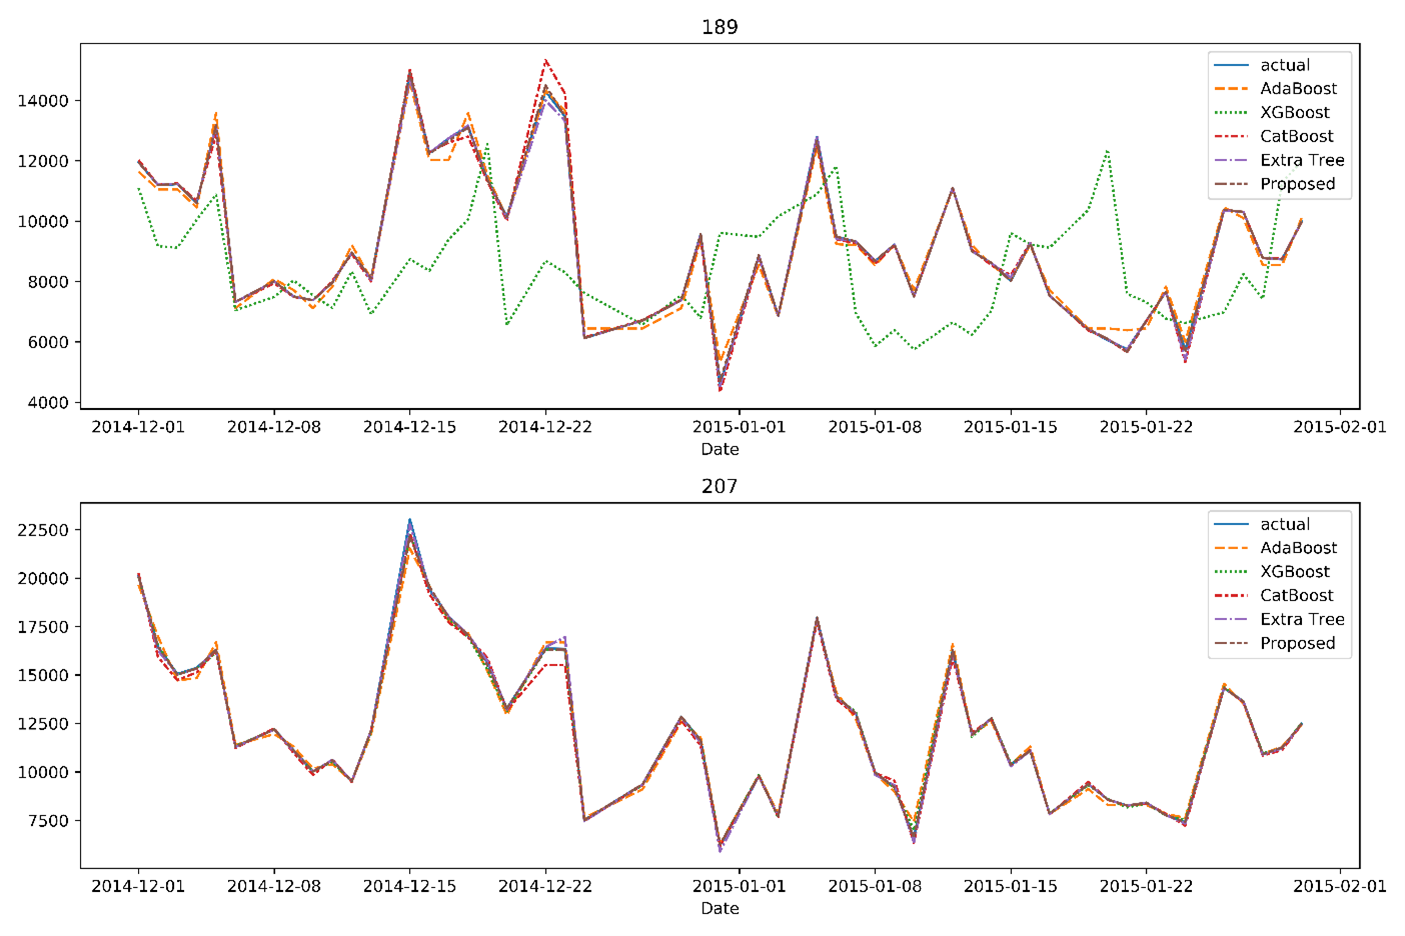
\includegraphics[scale=0.8]{Picture2_2.png}
 \label{}
 \caption{Prediction plot for Store 189 and 207}
% \end{flushleft}
\end{figure*}

\begin{figure*}[!h]
 %\begin{flushleft}
 \centering
 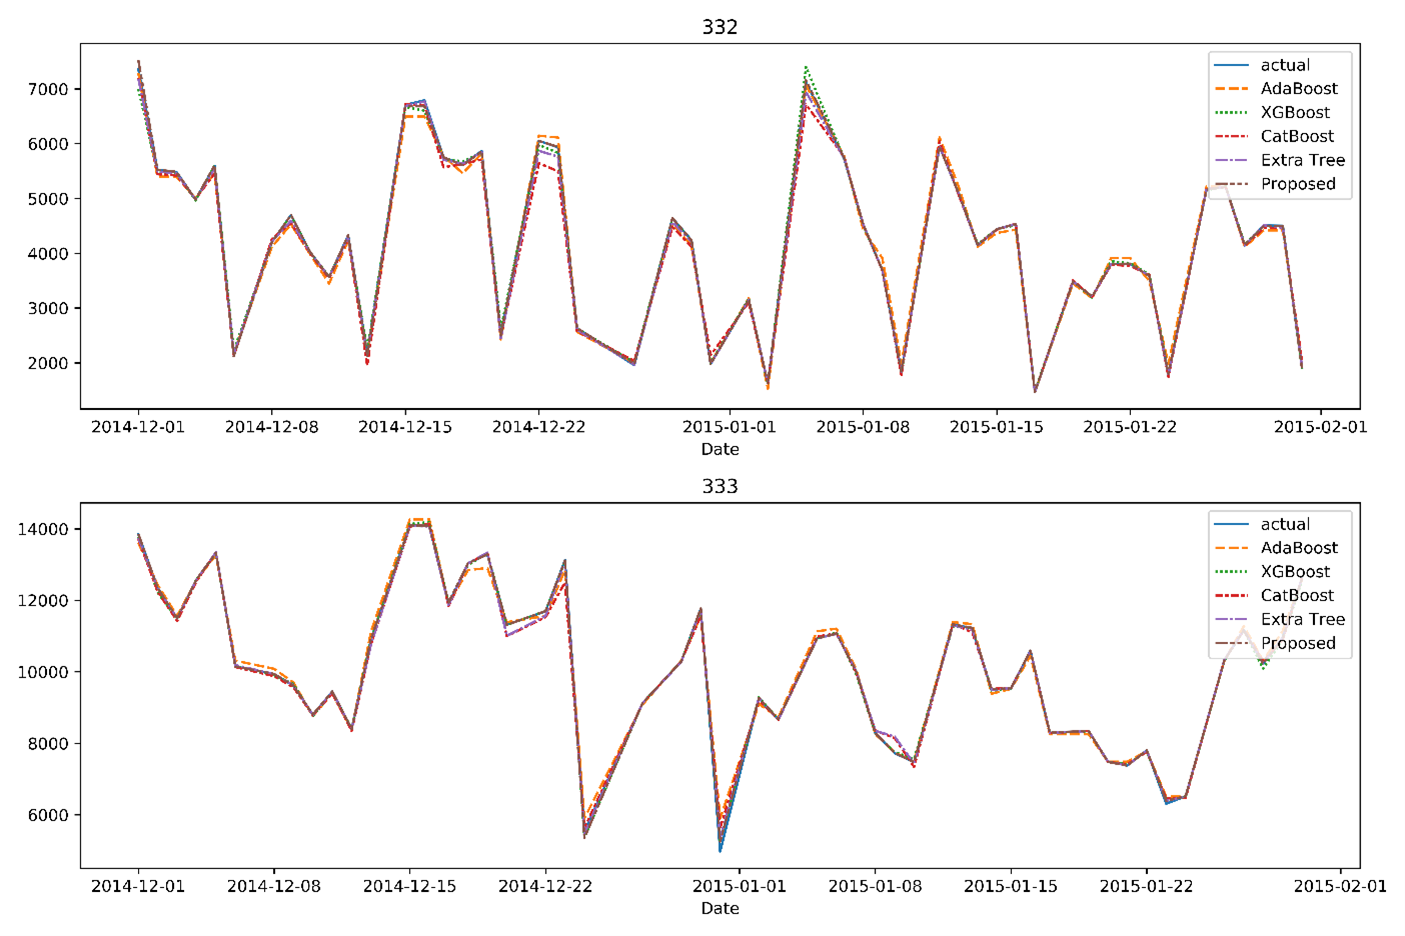
\includegraphics[scale=0.8]{Picture3.png}
 \label{}
 \caption{Prediction plot for Store 332 and 333}
% \end{flushleft}
\end{figure*}

\begin{figure*}[!h]
 %\begin{flushleft}
 \centering
 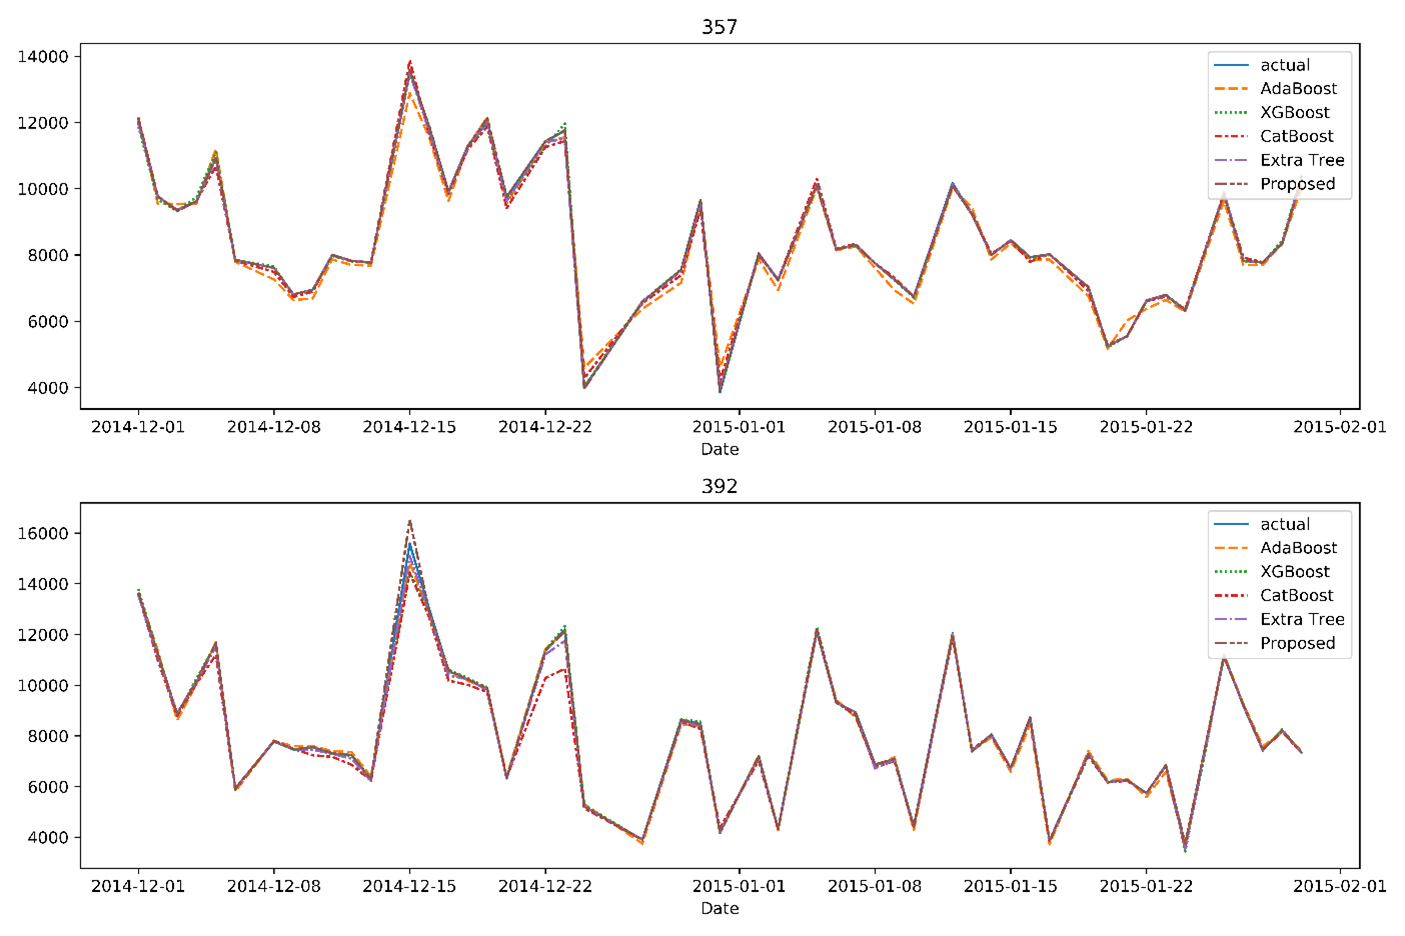
\includegraphics[scale=.8]{Picture4.png}
 \label{}
 \caption{Prediction plot for Store 357 and 392}
% \end{flushleft}
\end{figure*}

\begin{figure*}[!h]
 %\begin{flushleft}
 \centering
 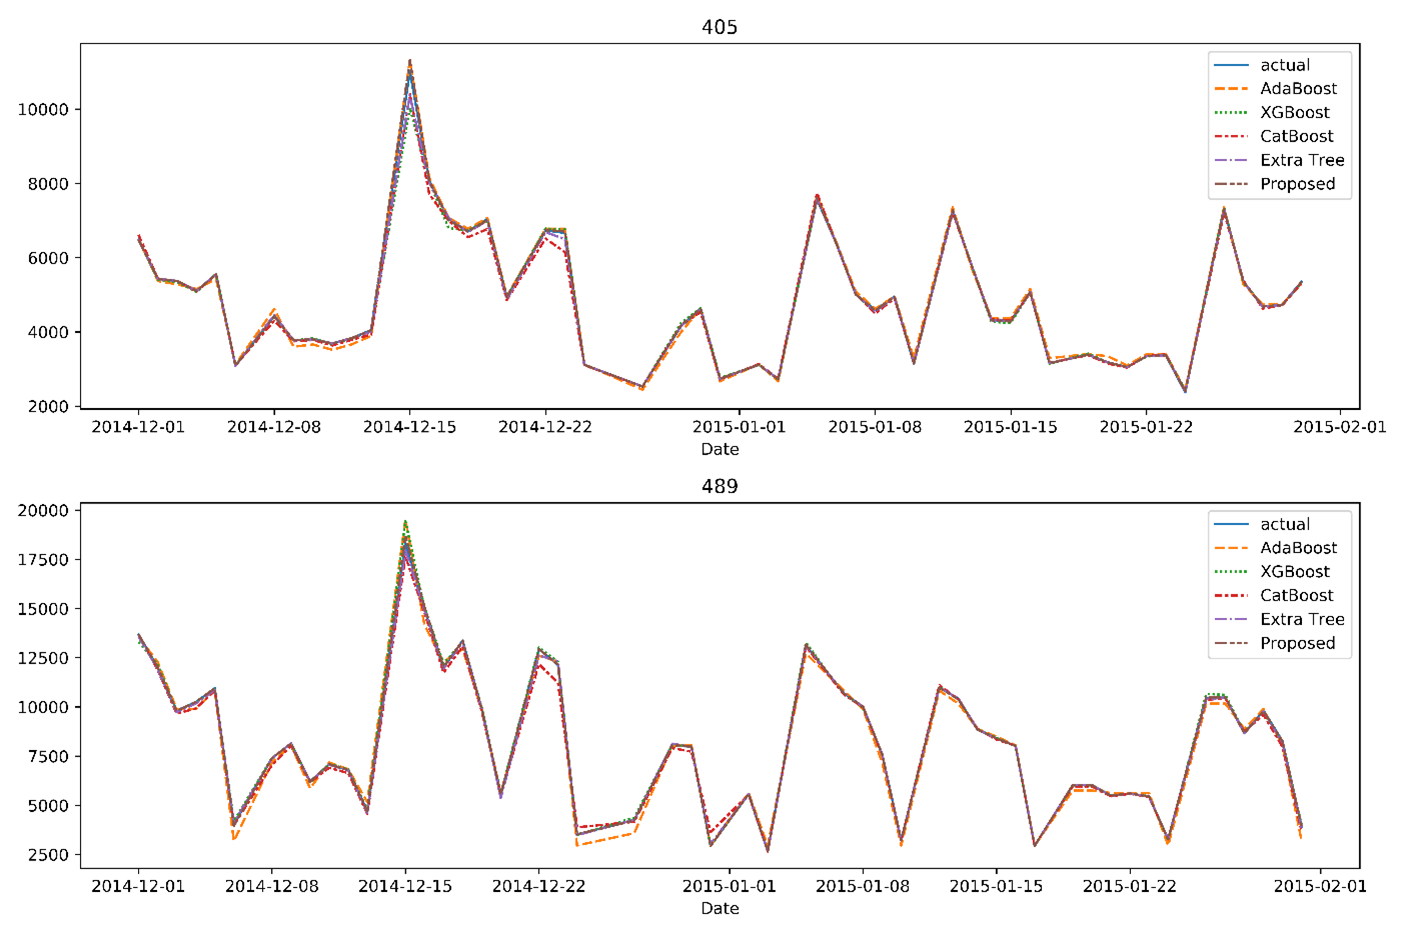
\includegraphics[scale=.8]{Picture5.png}
 \label{}
 \caption{Prediction plot for Store 405 and 489}
% \end{flushleft}
\end{figure*}

\begin{figure*}[!h]
 %\begin{flushleft}
 \centering
 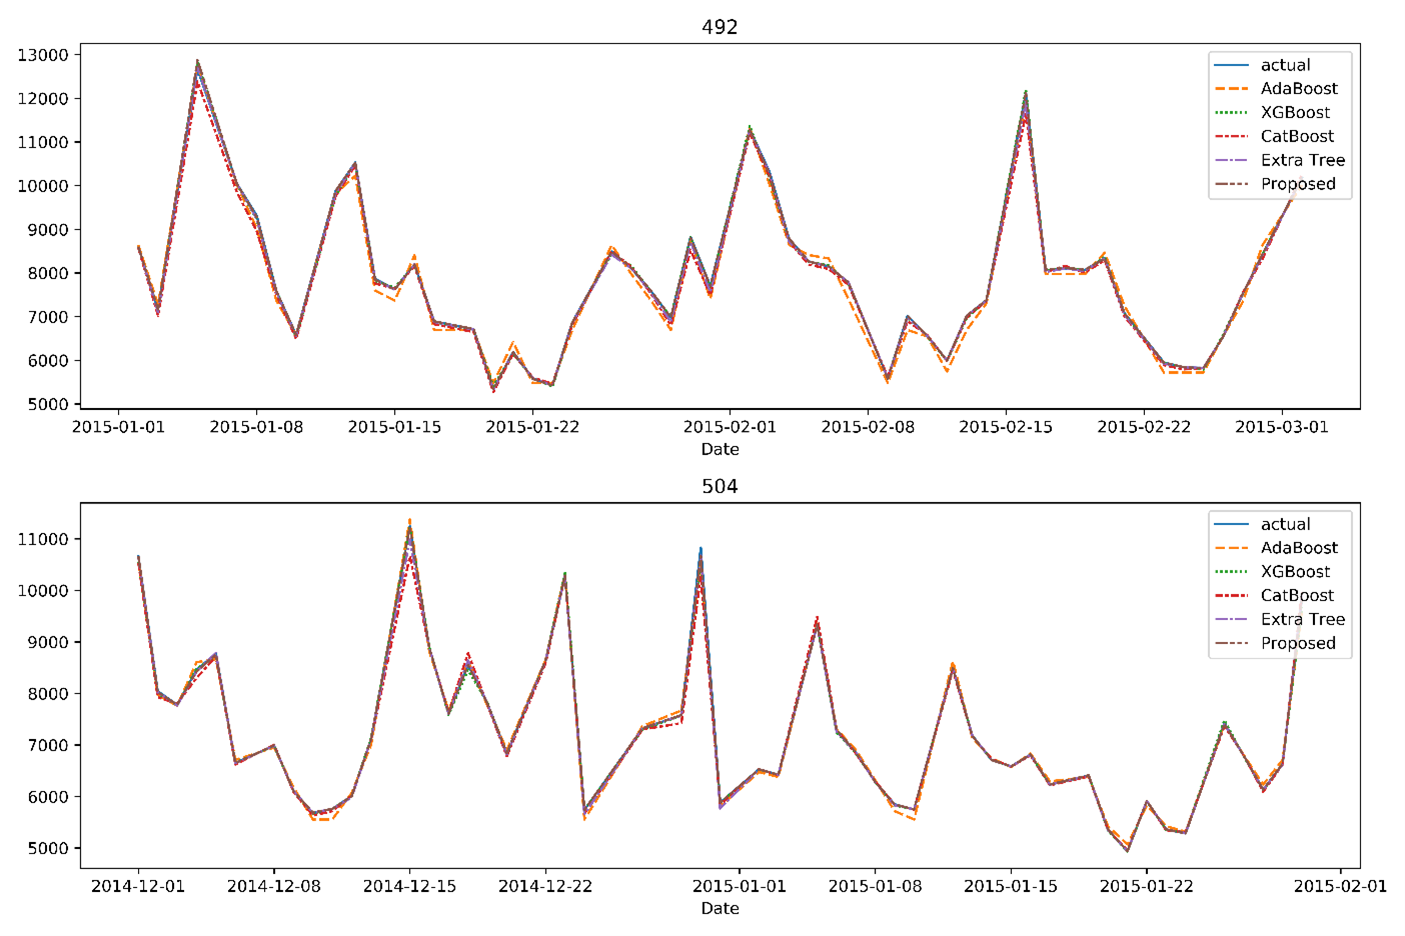
\includegraphics[scale=.8]{Picture6.png}
 \label{}
 \caption{Prediction plot for Store 492 and 504}
% \end{flushleft}
\end{figure*}


%PLOTTING
\begin{figure*}[!h]
 %\begin{flushleft}
 \centering
 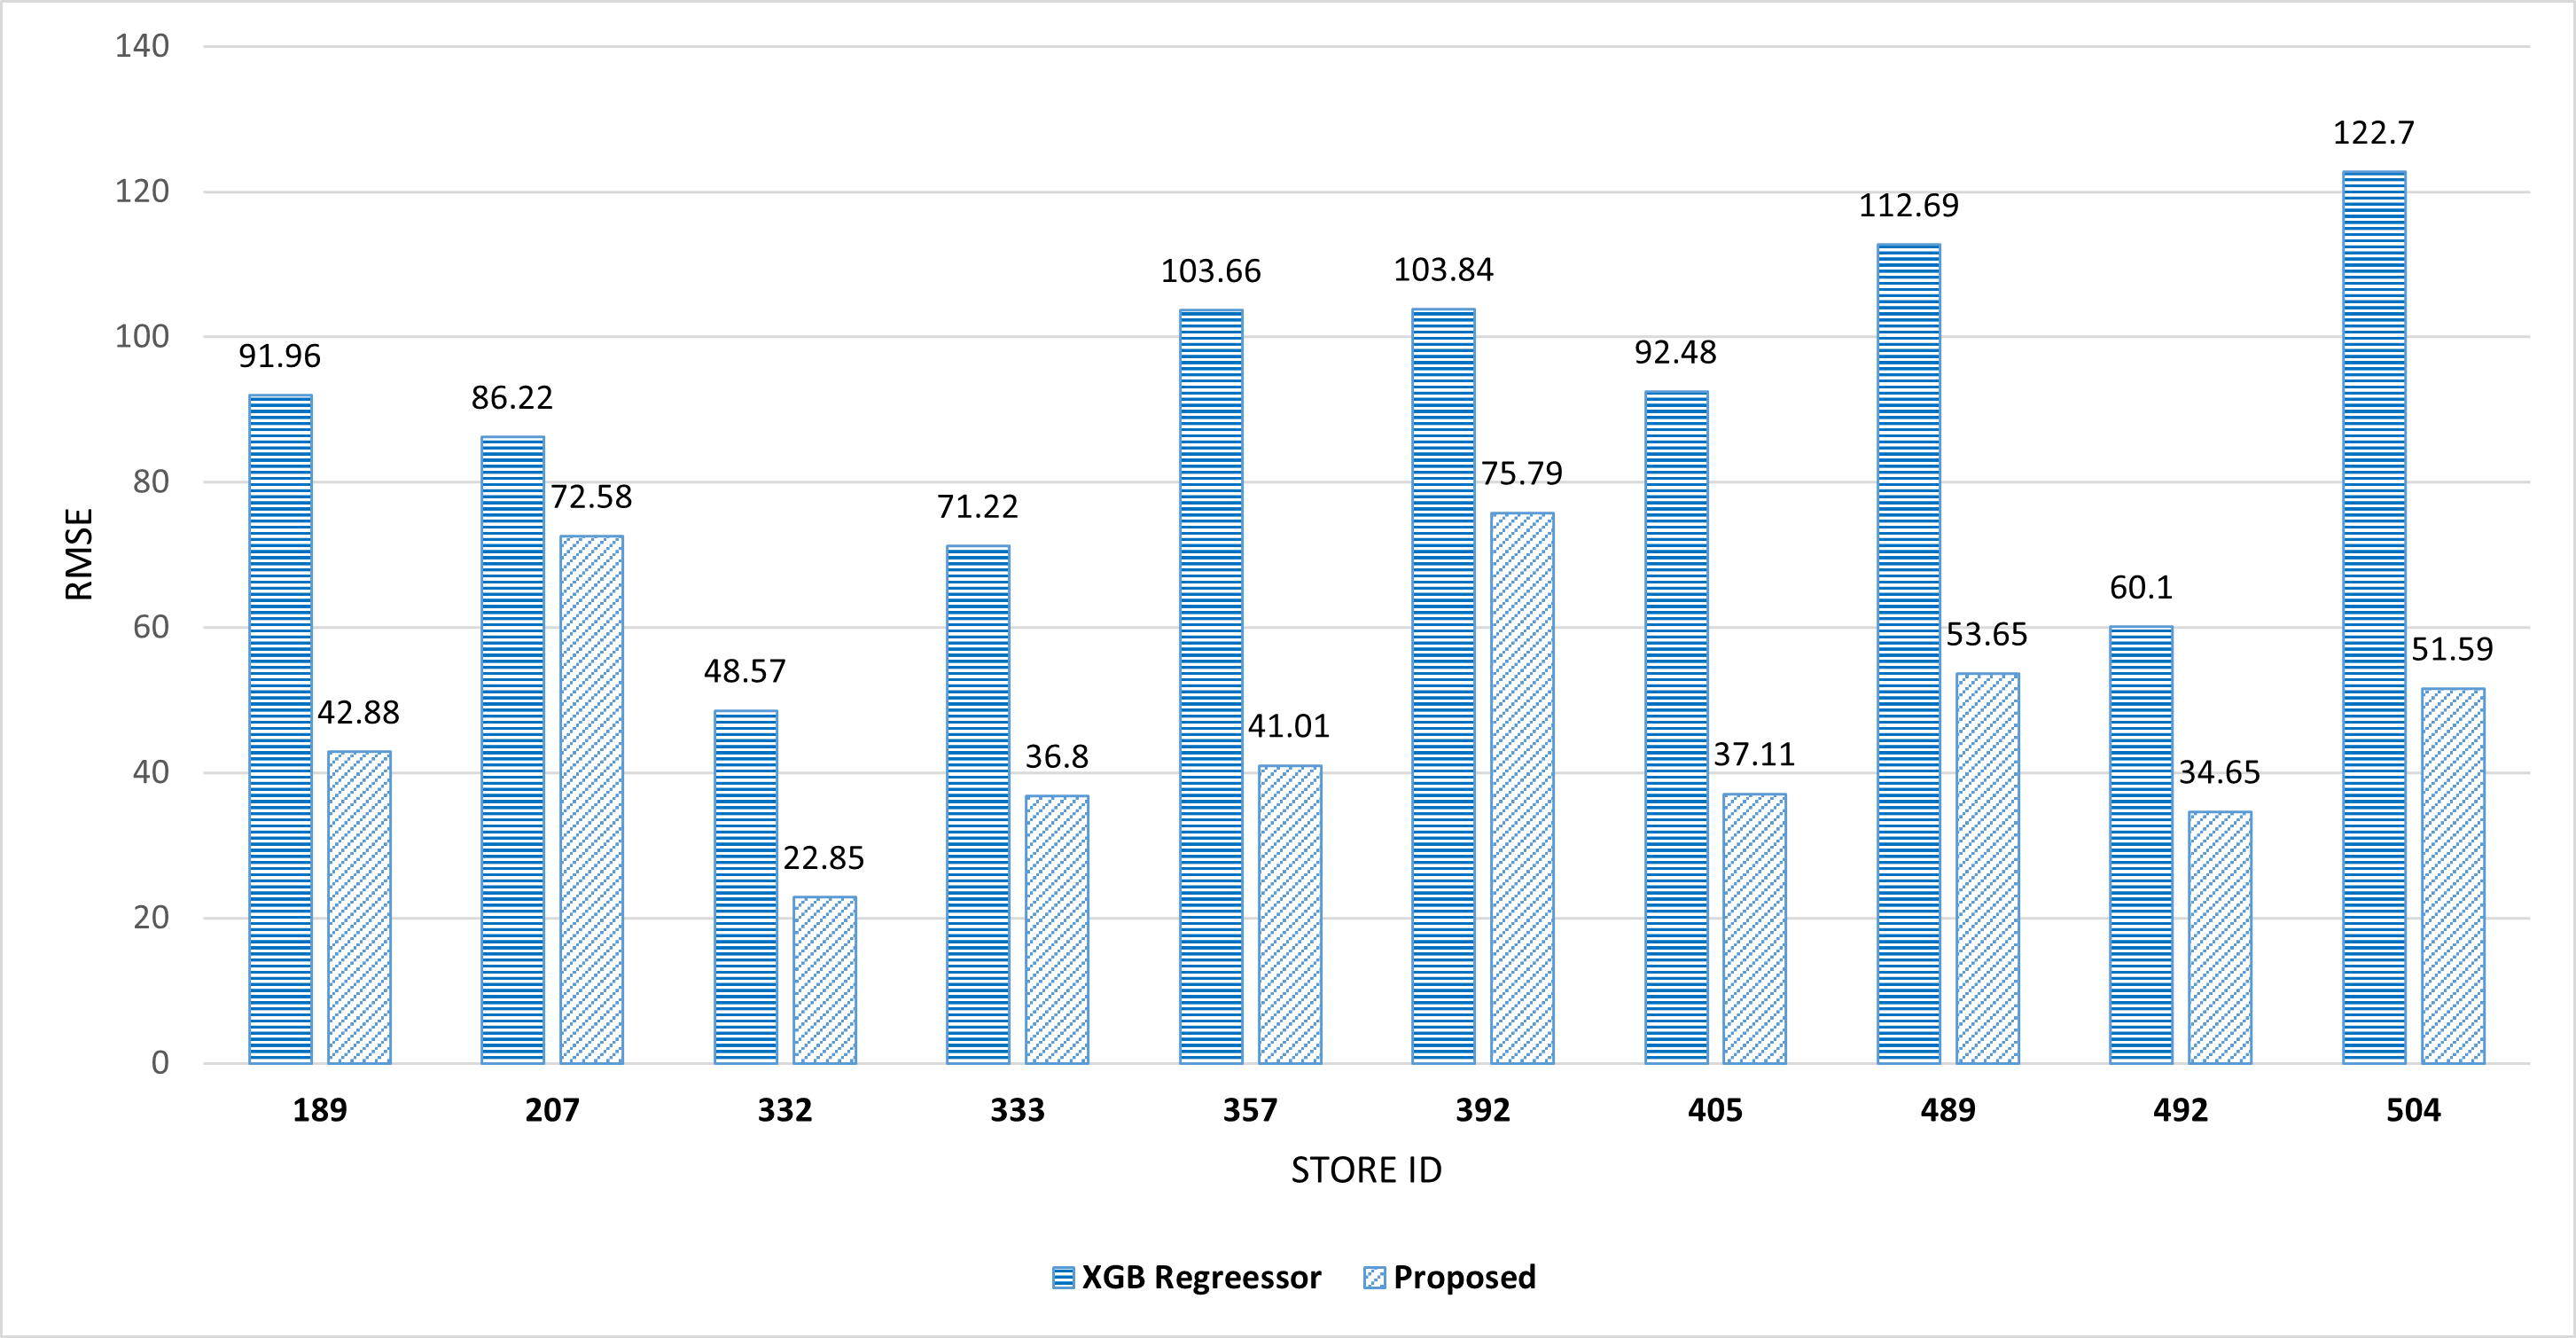
\includegraphics[scale=0.7]{xgb_p_plot1.png}
 \label{View Optimization}
 \caption{Comparative barplot of XGB Regressor and Proposed framework }
% \end{flushleft}
\end{figure*} 


\begin{figure*}[!h]
 %\begin{flushleft}
 \centering
 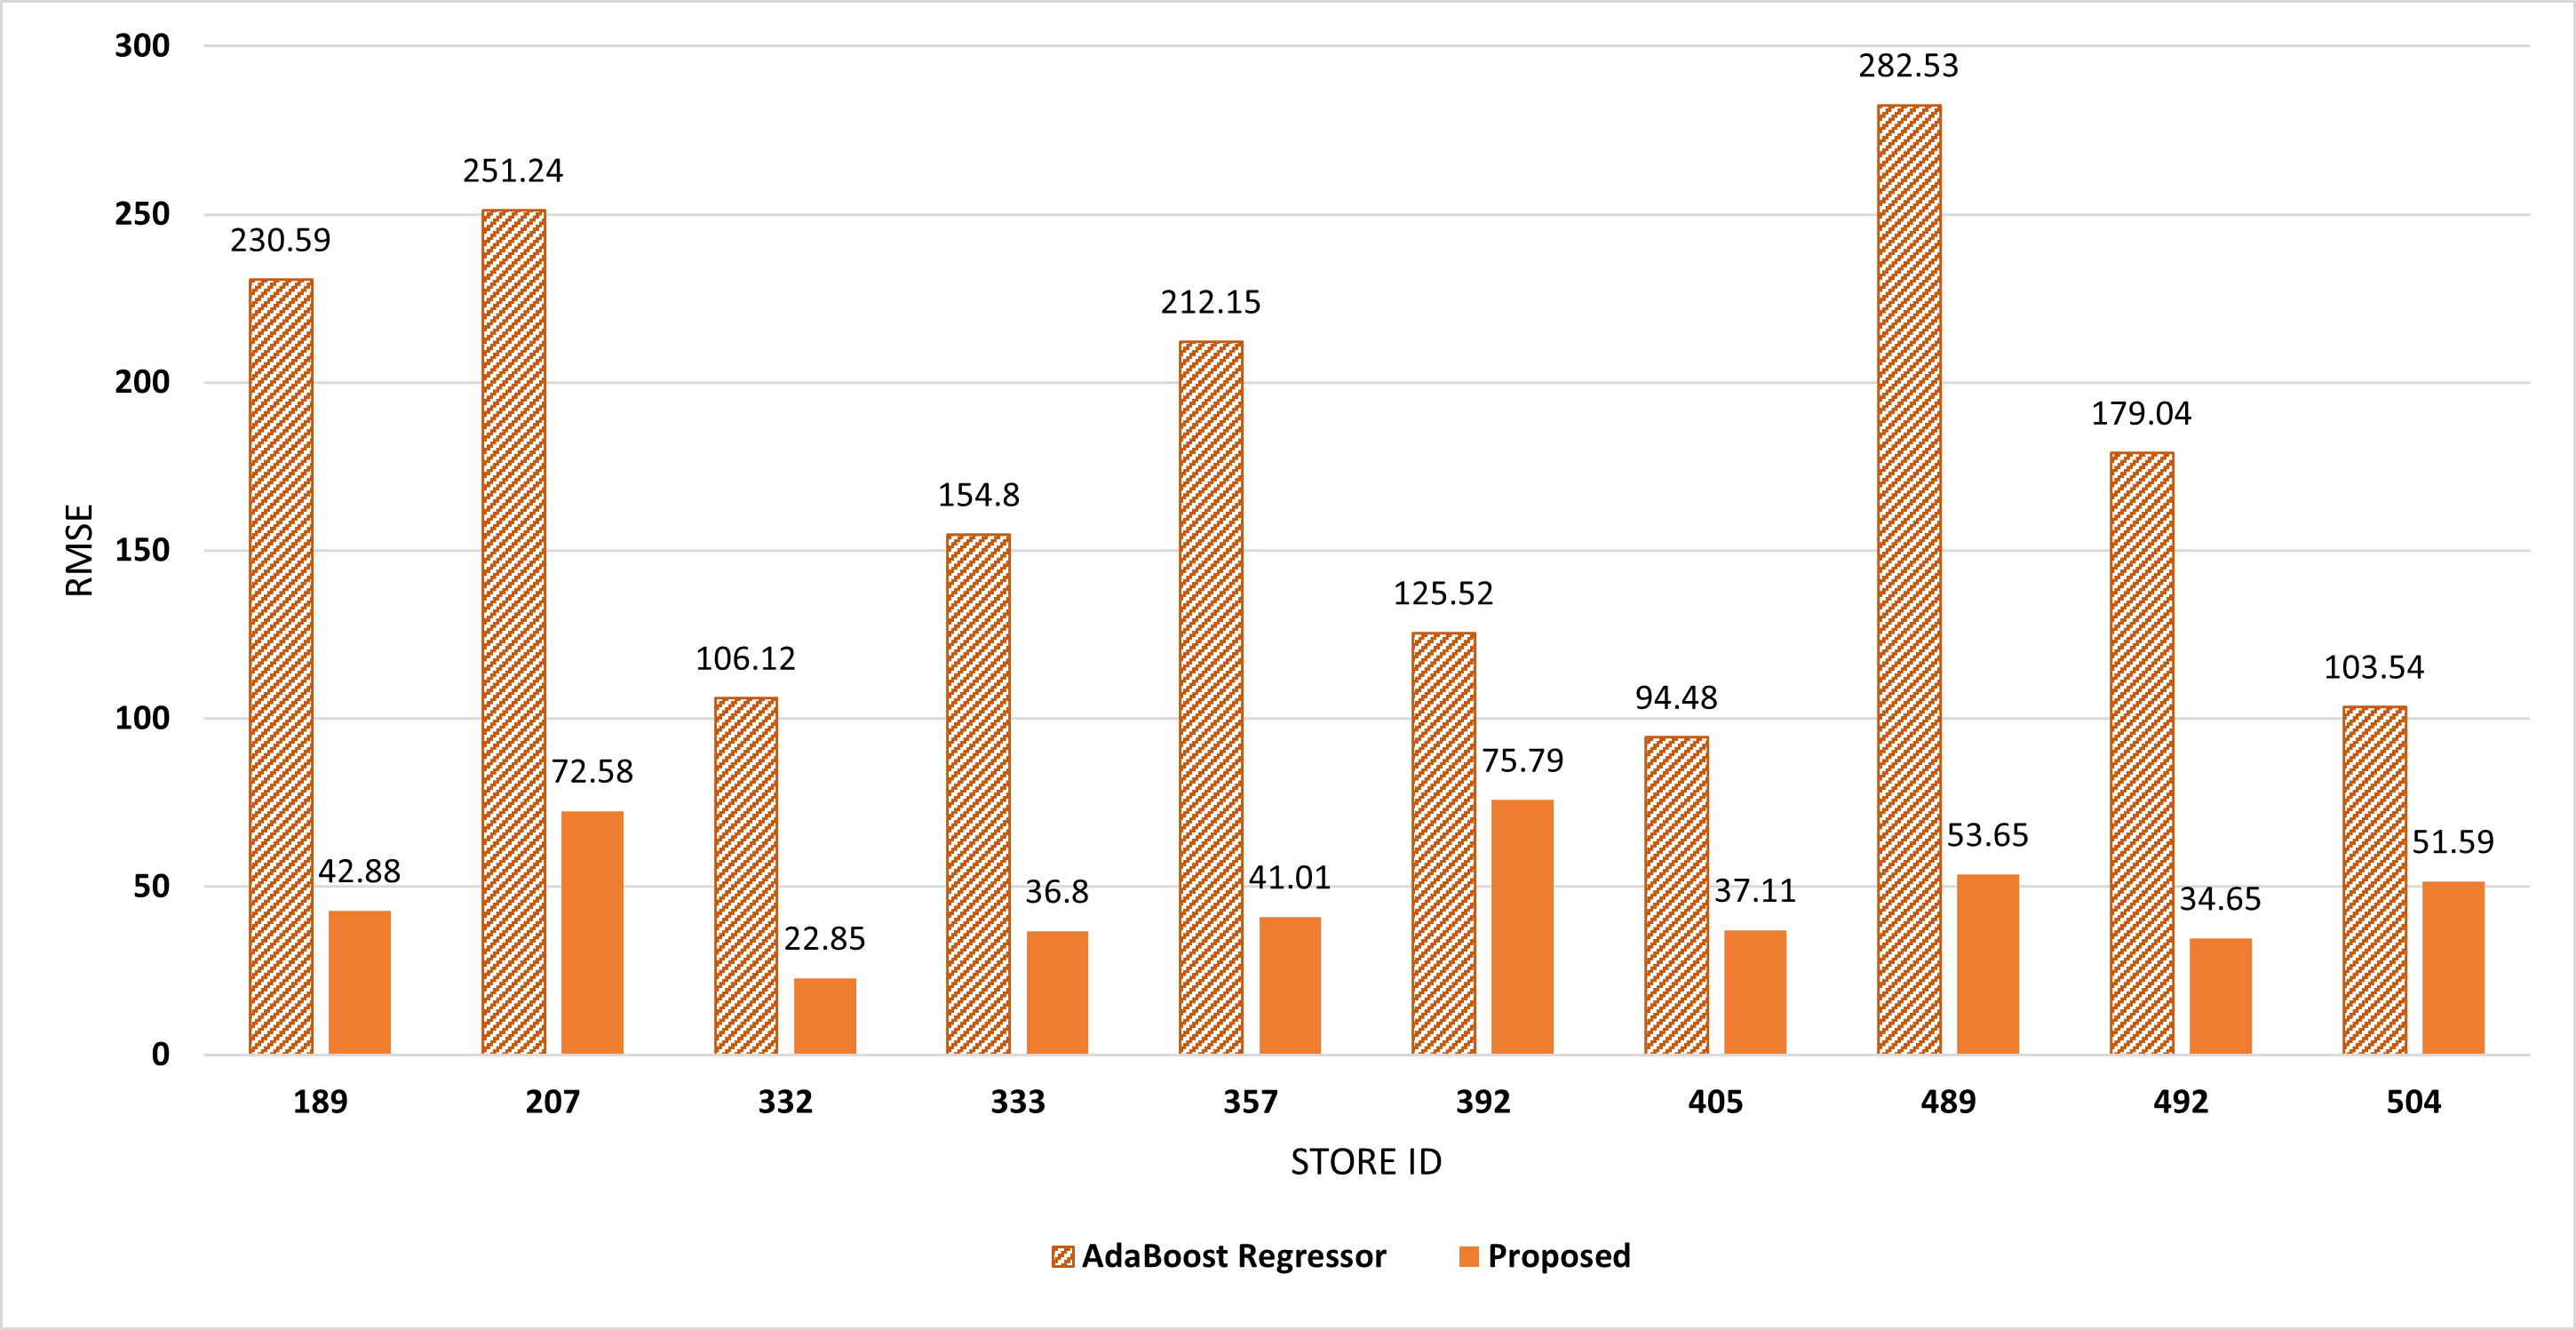
\includegraphics[scale=0.7]{adb_p_plot1.png}
 \label{View Optimization}
 \caption{Comparative barplot of AdaBoost Regressor and Proposed framework }
% \end{flushleft}
\end{figure*} 


\begin{figure*}[!h]
 %\begin{flushleft}
 \centering
 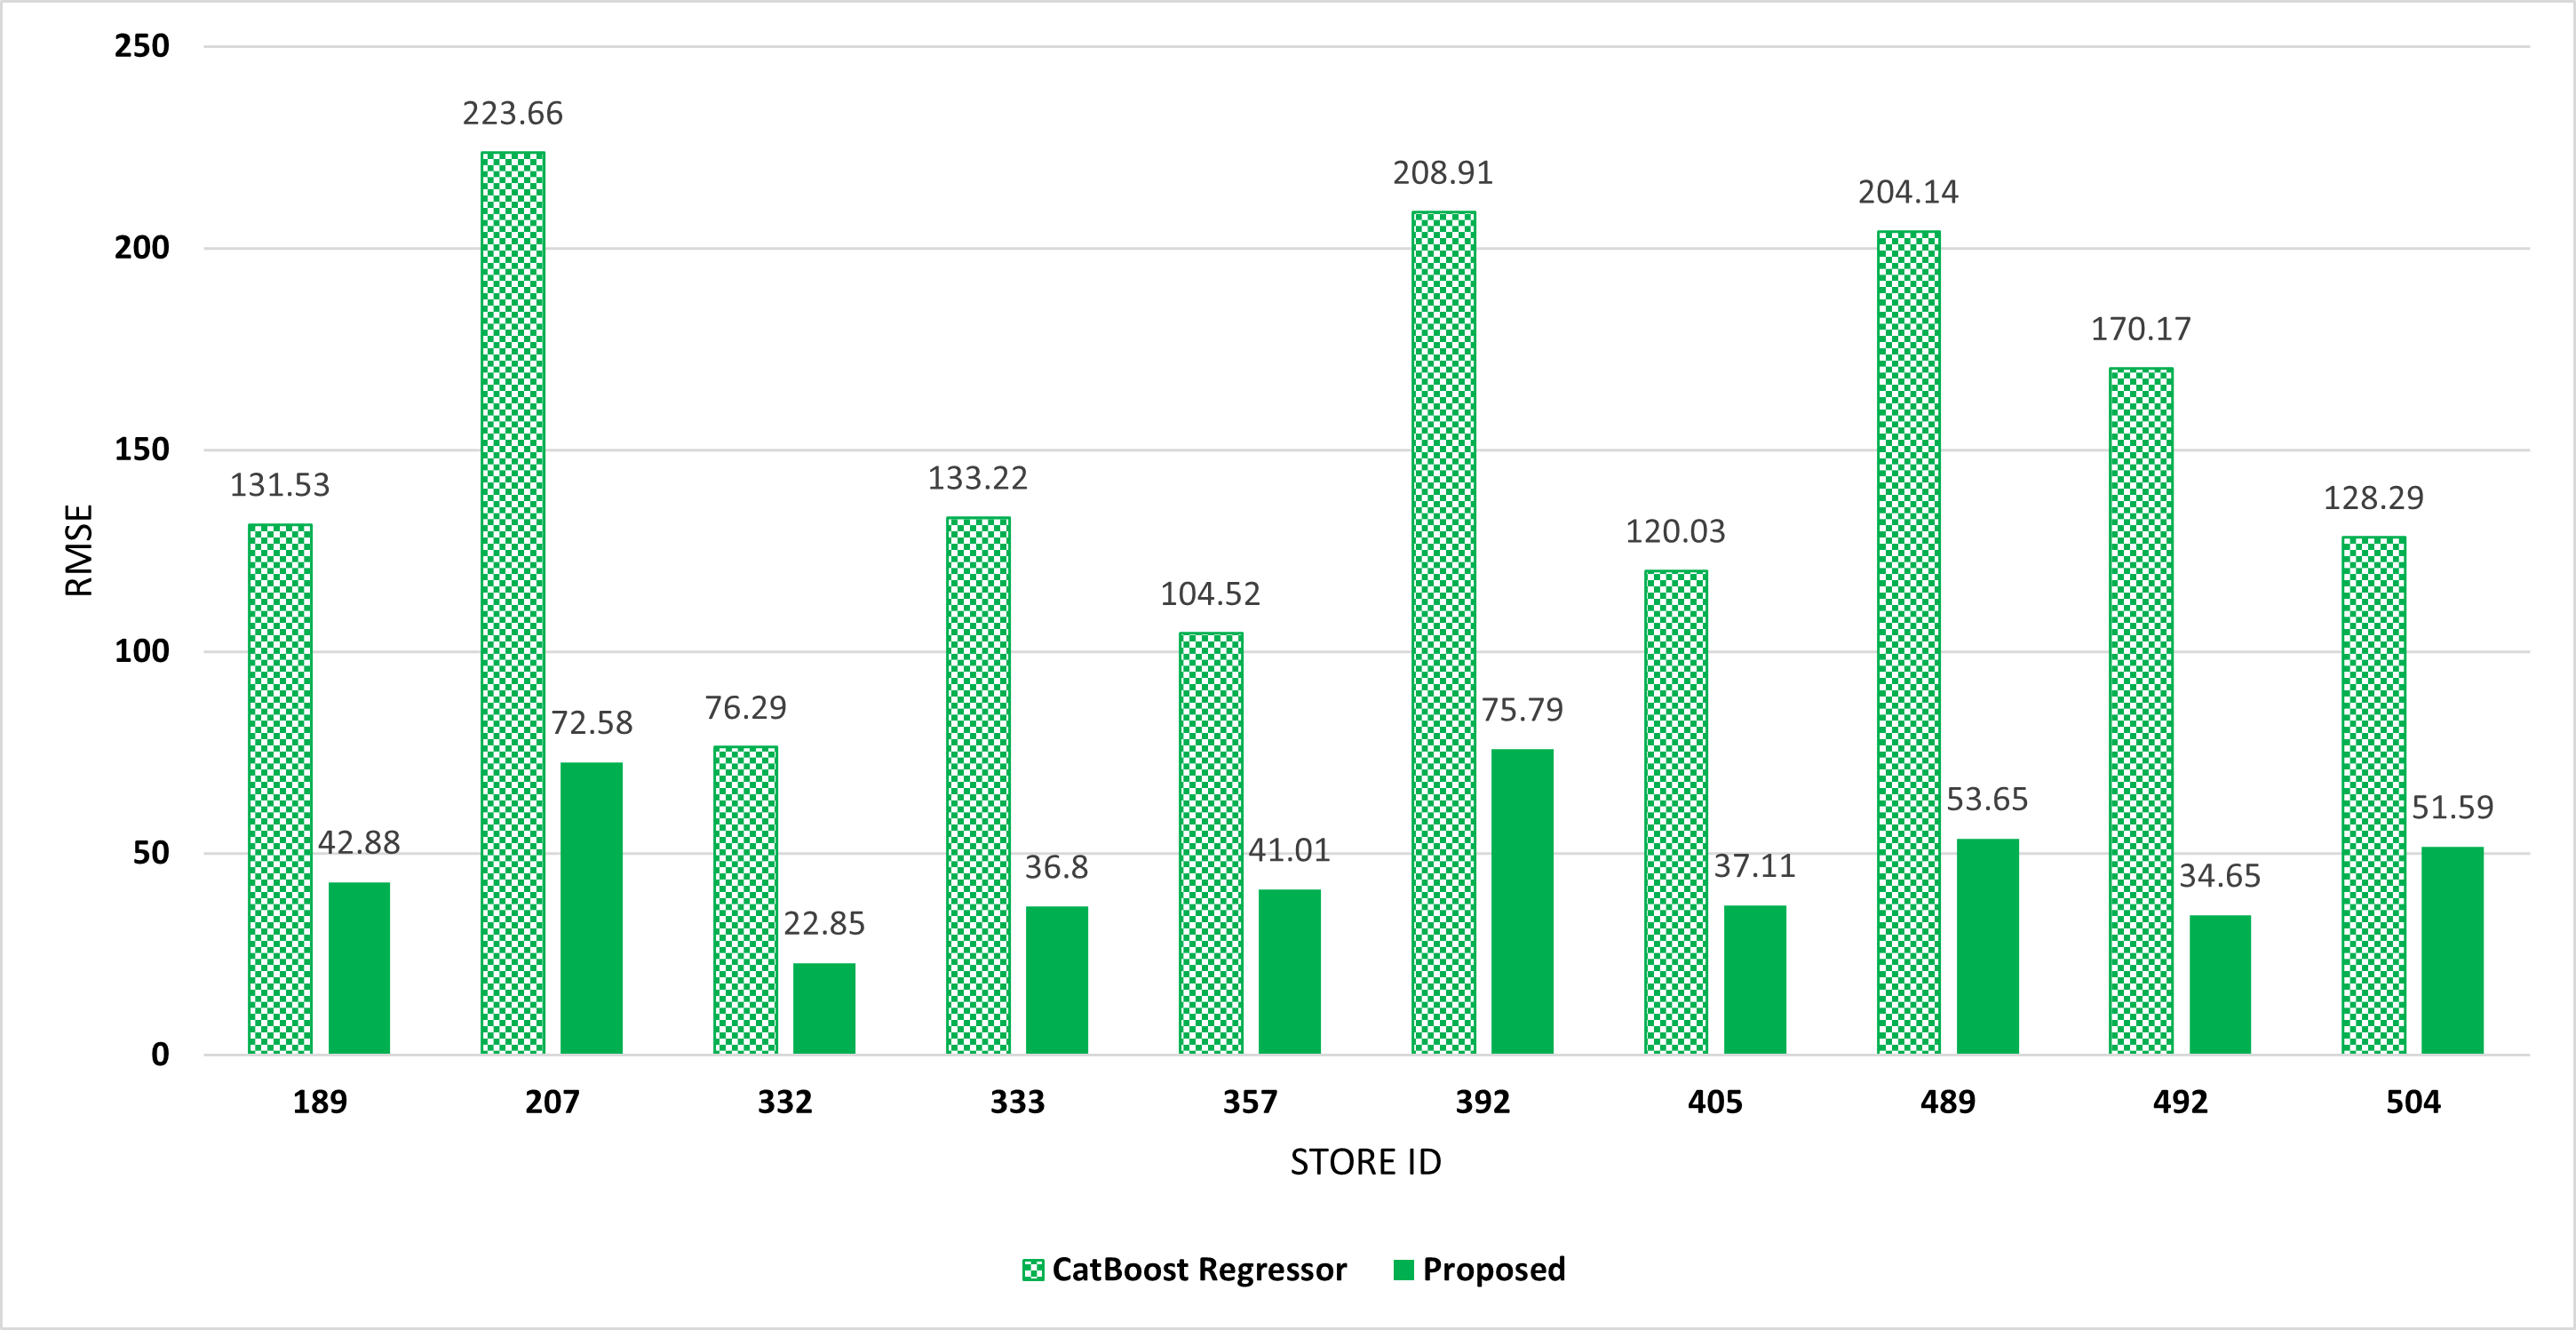
\includegraphics[scale=0.7]{catb_p_plot1.png}
 \label{}
 \caption{Comparative barplot of CatBoost Regressor and Proposed framework }
% \end{flushleft}
\end{figure*}

\begin{figure*}[!h]
 %\begin{flushleft}
 \centering
 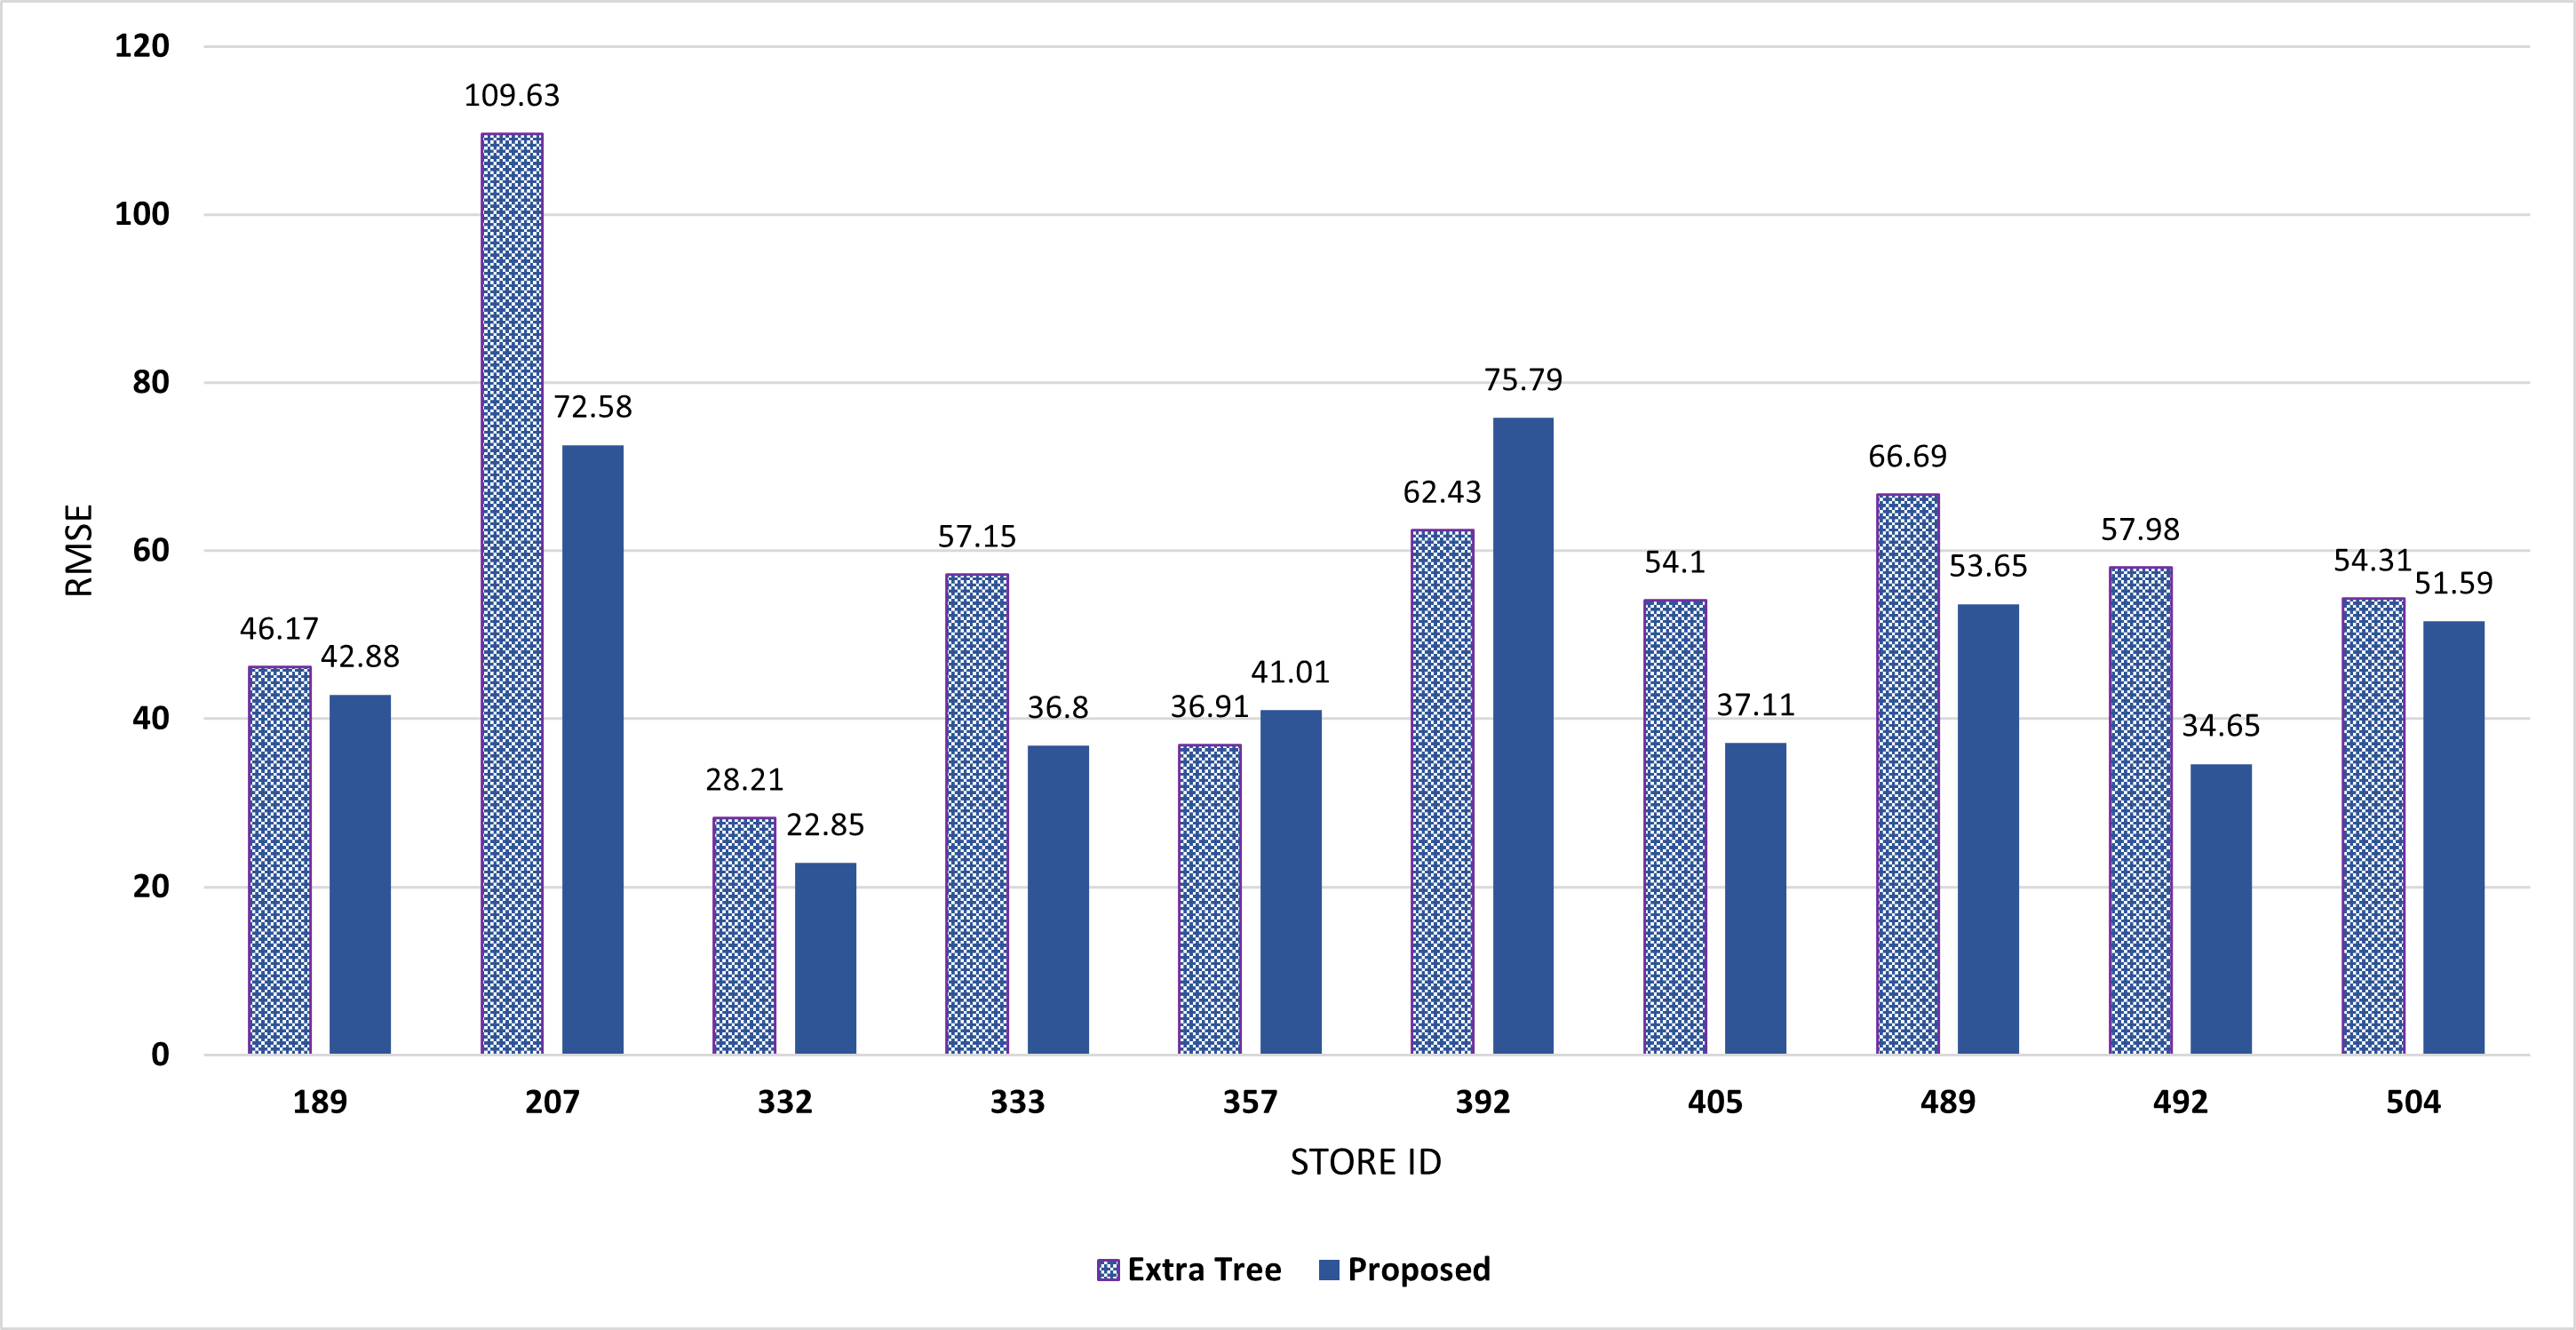
\includegraphics[scale=0.7]{extra_p_plot1.png}
 \label{}
 \caption{Comparative barplot of Extra Tree and Proposed framework }
% \end{flushleft}
\end{figure*}



%HYPERPARAMETER TABLE
% Please add the following required packages to your document preamble:
% \usepackage{multirow}
% \usepackage{graphicx}
\begin{table*}[]
\centering
\setlength{\tabcolsep}{3pt}
 {\renewcommand{\arraystretch}{1}%
\caption{Hyperparameters used}
\label{tab:my-table}
%\resizebox{\textwidth}{!}{%
\begin{tabular}[c]{|p{0.3\textwidth}|p{0.3\textwidth}|p{0.3\textwidth}|}
\hline   \textbf{Model}                & \textbf{Parameters} & \textbf{Value}  \\ \hline 
\multirow{4}{*}{XGBoost   Regressor}  &  Training data       & \textless   “2014-12”                \\
                                      & n\_estimators       & 100                                  \\
                                      & learning\_rate      & 1.0                                  \\
                                      & verbose            & True                                \\  \hline 
\multirow{4}{*}{CatBoost   Regressor} & Training data       & \textless   “2014-12”                \\
                                      & random\_state       & 0                                    \\
                                      & learning\_rate      & 0.037556 ( default set   by system ) \\
                                      & n\_estimtors        & Default value   set automtically     \\ \hline
\multirow{4}{*}{AdaBoost   Regressor} & Training data       & \textless   “2014-12”                \\
                                      & random\_state       & 0                                    \\
                                      & n\_estimators       & 50    (default value)                \\
                                      & learning\_rate      & 1.0   (default value )               \\  \hline
\multirow{3}{*}{Extra Tree}           & Training data       & \textless   “2014-12”                \\
                                      & n\_estimators       & 100                                  \\
                                      & random\_state       & 0       \\ \hline
\end{tabular}%

}
\end{table*}



\subsection{Non-parametric Test}
Friedman ranking system is an approach to establish a comparison between different models. We cannot expect every model to work well in all circumstances. It is achieved through a test known as Friedman Test. No single technique is applicable to all problems. Rather, what we have is a bag of tools and a bag of problems.\cite{zimmerman1993relative} Friedman test can be defined as non-parametric statistical test which is robust to outliers. Apart from model validation, Friedman ranking has wide applications on other fields as well. The Friedman rank test (Friedman 1937) is appropriate for testing the null hypothesis that ordinal data from k matched samples are drawn from the same population or in situations where multiple correlated measures are obtained on the same subjects. This test is an alternative to the F-test for two-way analysis of variance when there is reason to believe that the assumptions underlying the classical ANOVA are not satisfied by the data. The data are arranged in a two-way table having N rows and k columns. The rows correspond to the blocks of matched subjects, and the columns represent the different treatments or experimental conditions. The values in the rows are the ranks of the scores for the different subjects under each of the k treatments. The ranks in a row range from 1 to k \cite{martin1993tables}\\

\begin{figure*}[!h]
 %\begin{flushleft}
 \centering
 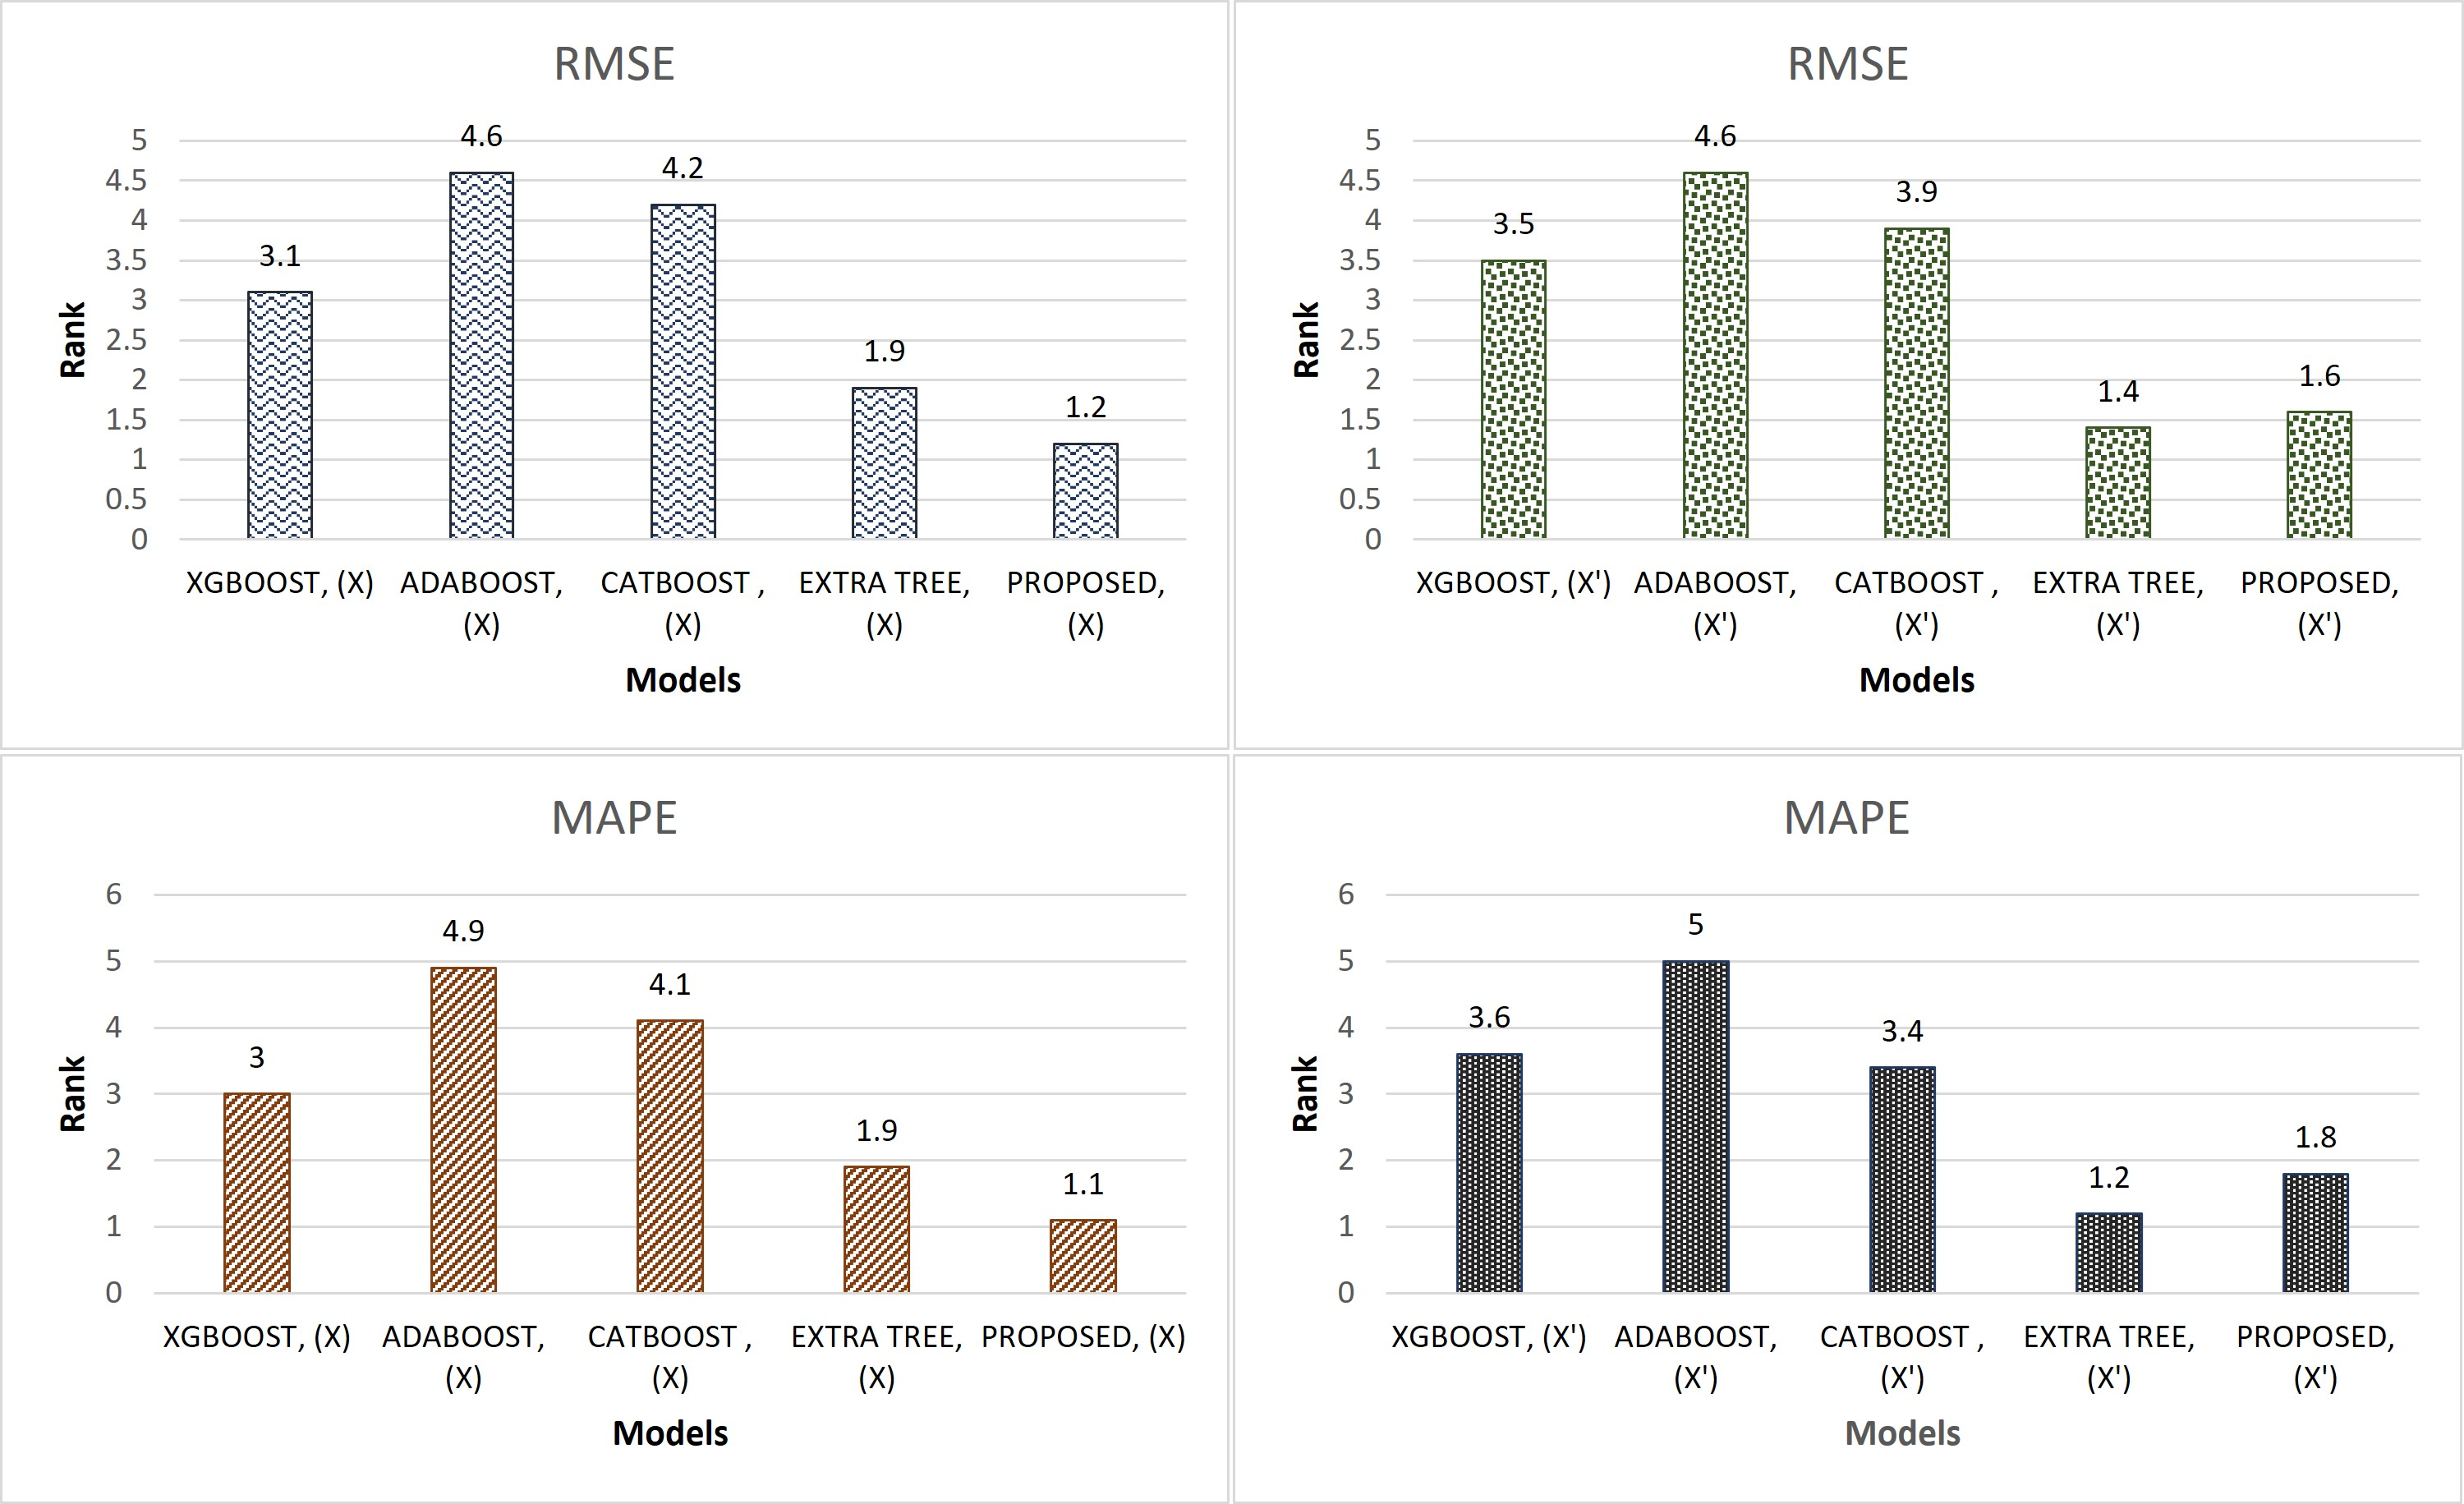
\includegraphics[scale=.68]{newc.jpg}
 \label{}
 \caption{Friedman Ranking plots for dataset category X and X' }
% \end{flushleft}
\end{figure*}


